\chapter{Getting Rich Is Easy}

This chapter follows a Jim Rohn lecture preserved through a curated LazyingArt LLC playlist. No validated board frames survive for this talk, so the mathematics has to be reconstructed from the spoken sequence itself. The lecture nevertheless has a clear spine. It begins with a paradox, then organizes itself into three reasons, then isolates the decisive variable by holding the outside world fixed, and finally compresses success and failure into a single distinction between doing and neglecting the easy things one can do.

\section{Easy, Hard, and the Three Reasons}

Rohn does not begin by proving anything. He begins by provoking us. He says that he got rich by the time he was thirty-one, and that it was easy. He briefly toys with the objection that it must have been hard, but he refuses to let go of the word ``easy.'' The chapter should preserve that tension. The later formulas matter because they are presented as an answer to this opening paradox.

He then imposes a clean structure on the lecture: there are three reasons. It is important to keep this counting device in the notes, because it governs the whole progression of the argument.

\begin{align}
\text{Reason 1} &= \text{I lived in America},\\
\text{Reason 2} &= \text{I found an opportunity},\\
\text{Reason 3} &= \text{I found a teacher}.
\end{align}

A compact reconstruction of the opening claim is therefore
\begin{equation}
\text{Rich by }31 \Longleftarrow E + O + T,
\end{equation}
where \(E\) stands for the favorable environment, \(O\) for opportunity, and \(T\) for the teacher. This is our shorthand, not Rohn's, but it captures the outer architecture of the lecture.

\section{America Is Easy}

The first reason is not a hidden trick, nor a financial instrument, nor an extraordinary talent. It is the field itself. Rohn says that he lived in America, and then he repeats the proposition that America is easy. The repetition is not ornamental. He is trying to fix a background condition before he turns to personal action.

\begin{equation}
\text{America}=\text{easy}.
\end{equation}

The claim is developed by contrast rather than by formal analysis. Bangladesh is hard; Cambodia is hard; India is hard; China is really hard. The lecture is not giving a theory of comparative development. It is trying to impress on the listener that the surrounding environment is unusually permissive.

\subsection{Question \& Answer}

\paragraph{Question.} What is the first reason he gives for getting rich by thirty-one?

\paragraph{Answer.} He places the first reason outside himself. He lived in America, and for the purposes of this lecture that means he began in an environment full of openings rather than one closed down by severe scarcity or political violence.

One can write the comparative rhetoric in stripped-down form as
\begin{align}
\text{America} &= \text{easy},\\
\text{Bangladesh} &= \text{hard},\\
\text{Cambodia} &= \text{hard},\\
\text{India} &= \text{hard},\\
\text{China} &= \text{really hard}.
\end{align}

The lecture then recaps: if we take one thing home from this first movement, it is simply that America is easy. Only after that baseline has been fixed does Rohn move to the second reason.

\section{Opportunity, Doors, and Trying Again}

Once the background has been established, Rohn asks what that environment is good for. His answer is opportunity. But he is careful here. Opportunity is not a single golden ticket. It is an iterative process of search, trial, failure, and renewed trial.

\begin{equation}
\text{America} \Longrightarrow \text{full of opportunity}.
\end{equation}

The lecture's operational chain is short and exact:
\begin{align}
\text{Search for an opportunity} &\Longrightarrow \text{Try it},\\
\text{One door closes} &\Longrightarrow \text{Another door opens},\\
\text{Try} &\Longrightarrow \text{Try again} \Longrightarrow \text{Try again}.
\end{align}

\subsection{Question \& Answer}

\paragraph{Question.} What do we do if the first opportunity is not the right one?

\paragraph{Answer.} We try it, and if it is not the one, we do not interpret the failure as the end of the matter. Another door opens. That, for Rohn, is part of what makes the country easy.

This iterative structure is worth preserving visually, even though no board frame survives:

\begin{figure}[h]
\centering
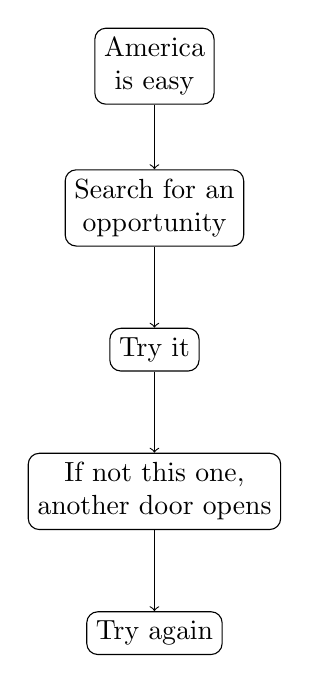
\begin{tikzpicture}
\node[draw, rounded corners, align=center] (a) at (0,0) {America\\is easy};
\node[draw, rounded corners, align=center] (b) at (0,-1.8) {Search for an\\opportunity};
\node[draw, rounded corners, align=center] (c) at (0,-3.6) {Try it};
\node[draw, rounded corners, align=center] (d) at (0,-5.4) {If not this one,\\another door opens};
\node[draw, rounded corners, align=center] (e) at (0,-7.2) {Try again};

\draw[->] (a) -- (b);
\draw[->] (b) -- (c);
\draw[->] (c) -- (d);
\draw[->] (d) -- (e);
\end{tikzpicture}
\caption{Transcript-derived opportunity chain. The lecture treats opportunity as iterative rather than singular.}
\end{figure}

This whole section leads naturally into the third reason. Environment gives openings, but openings by themselves do not yet explain transformation. That requires instruction.

\section{The Teacher and the Two Six-Year Blocks}

The third reason is the teacher. Rohn treats this as a decisive event, and he gives the teaching in two parts. First comes diagnosis: the years from nineteen to twenty-five were messed up. Then comes method: the next six years need not resemble the last six.

We can formalize the before-and-after structure as
\begin{align}
S_1 &= \text{first six years}=\text{messed up},\\
S_2 &= \text{second six years}=\text{millionaire}.
\end{align}

The lecture then becomes unexpectedly controlled. Rohn holds the outside variables approximately fixed:
\begin{align}
G_2 &\approx G_1, & I_2 &\approx I_1,\\
W_2 &\approx W_1, & C_2 &\approx C_1,\\
Ec_2 &\approx Ec_1, & U_2 &\approx U_1,
\end{align}
where \(G\) is government, \(I\) interest rates, \(W\) wage scale, \(C\) circumstances, \(Ec\) economy, and \(U\) union philosophy. These symbols are a note-writer's compression of his repeated phrase ``about the same.''

\subsection{Question \& Answer}

\paragraph{Question.} If the surroundings stayed about the same, why did the second six years produce a millionaire?

\paragraph{Answer.} Because the outside was not the decisive variable. The self was.

The worked update rule is the heart of the chapter:
\begin{equation}
X_{\text{out},2} \approx X_{\text{out},1},
\qquad
\Delta \text{self} \neq 0
\Longrightarrow
S_2 \neq S_1.
\end{equation}

Rohn states the conclusion in plain language: everything around him was about the same, but he was not the same. He changed.

\subsection{Question \& Answer}

\paragraph{Question.} Can anybody do this?

\paragraph{Answer.} Rohn's answer is yes, but he sharpens the point immediately: if one stays the same, then the next six years will resemble the last six. The invitation is real, but so is the warning.

This prepares the next block, in which he removes the audience's remaining faith in outside rescue.

\section{The Not-Much List}

Once the changed-self principle has been introduced, Rohn begins clearing away false hopes. He does so by building what he calls, in effect, a ``not much list.'' The method is repetitive on purpose. He proposes one external improvement after another and asks what it would do for future and fortune.

\subsection{Question \& Answer}

\paragraph{Question.} What difference would those outside improvements make?

\paragraph{Answer.} Not much. That is his answer for better relatives, lower prices, a slightly better economy, one political party or the other, and even someone else's plans for us.

In compressed form,
\begin{align}
\text{Positive relatives} &\Longrightarrow \text{not much},\\
\text{Lower prices} &\Longrightarrow \text{not much},\\
\text{Better economy} &\Longrightarrow \text{not much},\\
\text{Democrats in power} &\Longrightarrow \text{not much},\\
\text{Republicans in power} &\Longrightarrow \text{not much},\\
\text{Someone else's plans for you} &= \text{not much}.
\end{align}

What this section accomplishes is not cynicism. It is variable elimination. The lecture is removing weak causes one by one. Hence the conclusion:
\begin{equation}
\text{Difference in future and fortune} \Longleftarrow \text{you make the difference}.
\end{equation}

Only after the outer list has been exhausted does the lecture deliver its central promise.

\section{Change Yourself First}

Now we get the promise from the teacher, which is one of the cleanest relations in the whole talk:
\begin{equation}
\text{If you change} \Longrightarrow \text{everything changes for you}.
\end{equation}

Rohn is careful to say what this does \emph{not} mean. We do not have to change government, prices, or taxes. The first change is elsewhere.

\subsection{Question \& Answer}

\paragraph{Question.} What has to change first?

\paragraph{Answer.} Philosophy. The lecture explicitly says that the first thing to change is the philosophy with which we face the world.

So the internal chain begins
\begin{align}
\text{First change} &= \text{your philosophy},\\
\text{Change philosophy}
&\Longrightarrow
\text{change mind, thought, information, knowledge, decisions}.
\end{align}

From there the consequences spread outward again. Health changes. Family relations change. Income and promotions change. The lecture does not supply a formal dynamical system, but its logic is plainly downstream: philosophy first, results later.

Rohn then replaces one final bad habit of thought. We do not wish for a better wind. We wish for the wisdom to set a better sail.

\subsection{Question \& Answer}

\paragraph{Question.} Should we wish for a better wind or learn to set a better sail?

\paragraph{Answer.} The wind stands for the outside world, the condition we do not command. The sail stands for preparation, judgment, and direction. The lecture insists that wisdom belongs on the side of the sail.

This relation can be written compactly as
\begin{align}
\text{Better sail} &> \text{better wind},\\
\text{Use whatever wind blows} &\Longrightarrow \text{go where you want to go}.
\end{align}

At this point the lecture has finally earned the right to return to its opening word, ``easy,'' and define it carefully.

\section{Easy to Do, Easy Not to Do}

Rohn now restages the original paradox, but with a new precision. ``Easy'' does not mean effortless. It means something he could do. The lecture inserts an important parenthesis here: he worked hard, got up early, stayed up late, and worked hard during those six years.

\begin{equation}
\text{Easy}=\text{something I can do}.
\end{equation}

This is a subtle but important definition. It separates the question of possibility from the question of labor. Something can be doable and still require sustained effort.

The obvious objection then arrives: if it was easy, why did everybody else not get rich?

\subsection{Question \& Answer}

\paragraph{Question.} If it was easy, why didn't everybody else get rich?

\paragraph{Answer.} Because the same things that are easy to do are also easy not to do.

That is the lecture's cleanest formula:
\begin{equation}
\text{Easy to do}=\text{easy not to do}.
\end{equation}

And the split between success and failure follows at once:
\begin{equation}
\text{Difference between success and failure}
\Longleftarrow
\text{easy to do / easy not to do}.
\end{equation}

Rohn then compresses his own story into one line:
\begin{equation}
\text{Fortune}
\Longleftarrow
\text{I did not neglect to do the easy things I could do every day for six years}.
\end{equation}

That line turns the whole lecture from biography into method. The positive name for success is non-neglect; the negative name for failure is neglect.

\subsection{Question \& Answer}

\paragraph{Question.} What is the major reason for not having more of what you want?

\paragraph{Answer.} Neglect.

The lecture then expands this into a cascade:
\begin{align}
\text{Neglect} &\Longrightarrow \text{infection} \Longrightarrow \text{disease},\\
\text{One neglect} &\Longrightarrow \text{another} \Longrightarrow \text{another}.
\end{align}

And the practical form of the disaster is stated with unusual clarity:
\begin{equation}
\text{Should do it}+\text{Could do it}+\text{Don't do it}
\Longrightarrow
\text{formula for disaster}.
\end{equation}

The same accumulation principle that produced fortune on the positive side now produces drift and ruin on the negative side:
\begin{equation}
\text{Six years of accumulated neglect}
\Longrightarrow
\text{undesired life, work, possessions, and self}.
\end{equation}

By the end of the section we see why the lecture had to be built in this order. The three reasons prepared the environment; the teacher isolated the variable; the promise shifted us inward; the word ``easy'' was then redefined; and only then could neglect emerge as the decisive difference.

\section{Summary}

This lecture begins as a paradox and ends as a discipline. Rohn first fixes the field: America is easy. He then adds opportunity and teacher. After that, however, the argument becomes sharper. Outer conditions remain about the same, yet the second six years differ from the first because the self changes. The ``not much list'' removes weak causes. Shoaff's promise relocates power inward, beginning with philosophy. The return to ``easy'' then resolves the opening tension: easy means something one can do, not something requiring no effort. Finally, the difference between success and failure is compressed into one choice, whether we do or neglect the easy things we could do.

The lecture can be summarized in two final relations. The first is the promise:
\begin{equation}
\text{If you change} \Longrightarrow \text{everything changes for you}.
\end{equation}

The second is the confession that makes the promise credible:
\begin{equation}
\text{Changed life} \Longleftarrow \text{it was me}.
\end{equation}

That is the whole movement of the chapter: field, opportunity, teacher, fixed outside, changed self, and then the long arithmetic of non-neglect.